\documentclass[12pt]{beamer}

\usepackage{caption}

\usepackage[utf8]{inputenc}



\usepackage[spanish]{babel}
%\usepackage{titlesec}

\usepackage{xcolor}
\usepackage{hyperref}%compilar 2 veces
\usepackage{geometry}
\usepackage{listings}
\usepackage{pdfpages}
\usepackage{subfig}%figuras una alado de otraa
\usepackage{float}


\usetheme{Copenhagen}

\usepackage{amsmath}
\usepackage{amsfonts}
\usepackage{amssymb}
\author{Angel Bejar Merma}
\title{Interface User Design}
%\setbeamercovered{transparent} 
%\setbeamertemplate{navigation symbols}{} 
%\logo{} 
\institute{Universidad Nacional de San Agustin} 
%\date{} 
%\subject{} 

\AtBeginSection[]
{
	\begin{frame}<beamer>{Contenido}
		\tableofcontents[currentsection,currentsubsection]
	\end{frame}
}


\begin{document}

\begin{frame}
\titlepage
\end{frame}

\begin{frame}{Contenido}


\tableofcontents
%\frametitle{contenido}
\end{frame}

\section{Concept}
\begin{frame}{concept}
User interface is the front-end application view to which user interacts in order to use the software .\\
User ser can manipulate and control the software
as well as hardware by means of user interface.

\end{frame}

\section{Part 1}
\begin{frame}{Part 1}
Today  user interface is found at almost every place where digital
technology exists right from computers mobile phones cars, music players,airplanes,ships etc.

\end{frame}


\begin{frame}
User interface is part of  software and is designed in such a way that it is -expected to provide the user insight of the software .\\
UI provides fundamental platform for human-computer interaction.
\\
-Ui can be graphical ,text-based ,audio-video based,depending upon the underlying hardware and software combination.\\
UI can be hardware or software or a combination of both.
\end{frame}


\begin{frame}{}



The software becomes more popular if its user interface
is:\\
\begin{block}


    \begin{itemize}
        \item Attractive
        \item Simple to use
        \item Responsive in short time
         \item Clear to understand
         \item Consistent on all interfacing screens
    \end{itemize}

\end{block}

\end{frame}

\begin{frame}
\begin{block}{UI broadly divided into two categories} 
 \begin{itemize}
\item command line interface

\item graphical user interface
\end{itemize}
\end{block}
\end{frame}

\section{Mapping User Objectives}




\begin{frame}{Mapping User Objectives}
\begin{figure}[H]
\centering
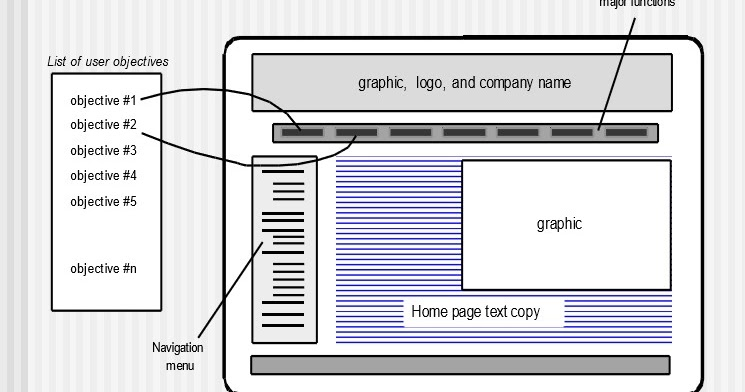
\includegraphics[width=10cm]{imagenes/diagrama2.jpg}
\caption{}
\end{figure}
\end{frame}

\section{Design Evaluation Cycle}

\begin{frame}{Design Evaluation Cycle}
\begin{figure}[H]
\centering
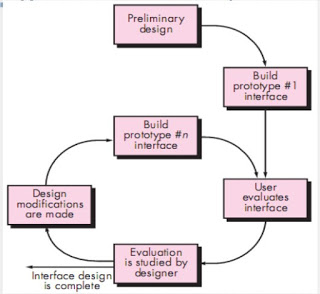
\includegraphics[width=8cm]{imagenes/evaluation.jpg}
\caption{}
\end{figure}
\end{frame}

\end{document}